\def\template{../template/}
\makeatletter \ifx\input@path\@undefined \def\input@path{{\template}} \else \g@addto@macro\input@path{{\template}} \fi \makeatother


% -- Documentclass --------------------------------------------------------%
\documentclass[english,pagenumoff]{rwth-document}
\usepackage{CAMMP-settings}

% -- Settings --------------------------------------------------------%
\setLogo{logo/cammp}
\setHeaderAsCAMMPweek
\setFooterAsCAMMPpartner

% Commands
\newcommand{\bs}{\boldsymbol}
\newcommand{\R}{\mathbb{R}}
\newcommand{\N}{\mathbb{N}}
\newcommand{\C}{\mathbb{C}}
\newcommand{\ephi}{\mathcal{E}_{\phi}^\xi}
\newcommand{\tphil}{\mathbb{T}_{\phi L}}
\newcommand{\eps}{\varepsilon}
\newcommand{\weak}{\rightharpoonup}
\newcommand{\weakstar}{\stackrel{\ast}{\rightharpoonup}}
\newcommand{\m}{\boldsymbol{m}}
\newcommand{\heff}{{\boldsymbol{h}}_{\text{eff}}}
\newcommand{\h}{\boldsymbol{H}}
\newcommand{\M}{\boldsymbol{M}}
\newcommand{\x}{\boldsymbol{x}}
\newcommand{\y}{\boldsymbol{y}}
\newcommand{\ra}{\rangle}
\newcommand{\la}{\langle}
\newcommand{\del}{\partial}
\newcommand{\dd}[2]{\frac{\partial #1}{\partial #2}}

% ----------------------------------------------------------%
\begin{document}
	
	\begin{center}
		{ \bfseries\LARGE Magnetic Domain-Wall Racetrack Memory}\\[1ex]
		Prof. Dr. C.\ Melcher (RWTH Aachen) \& Prof. Dr. S.\ Bl\"ugel (FZJ)
		%\\\scriptsize IVU Traffic Technologies AG
	\end{center}




\begin{center}
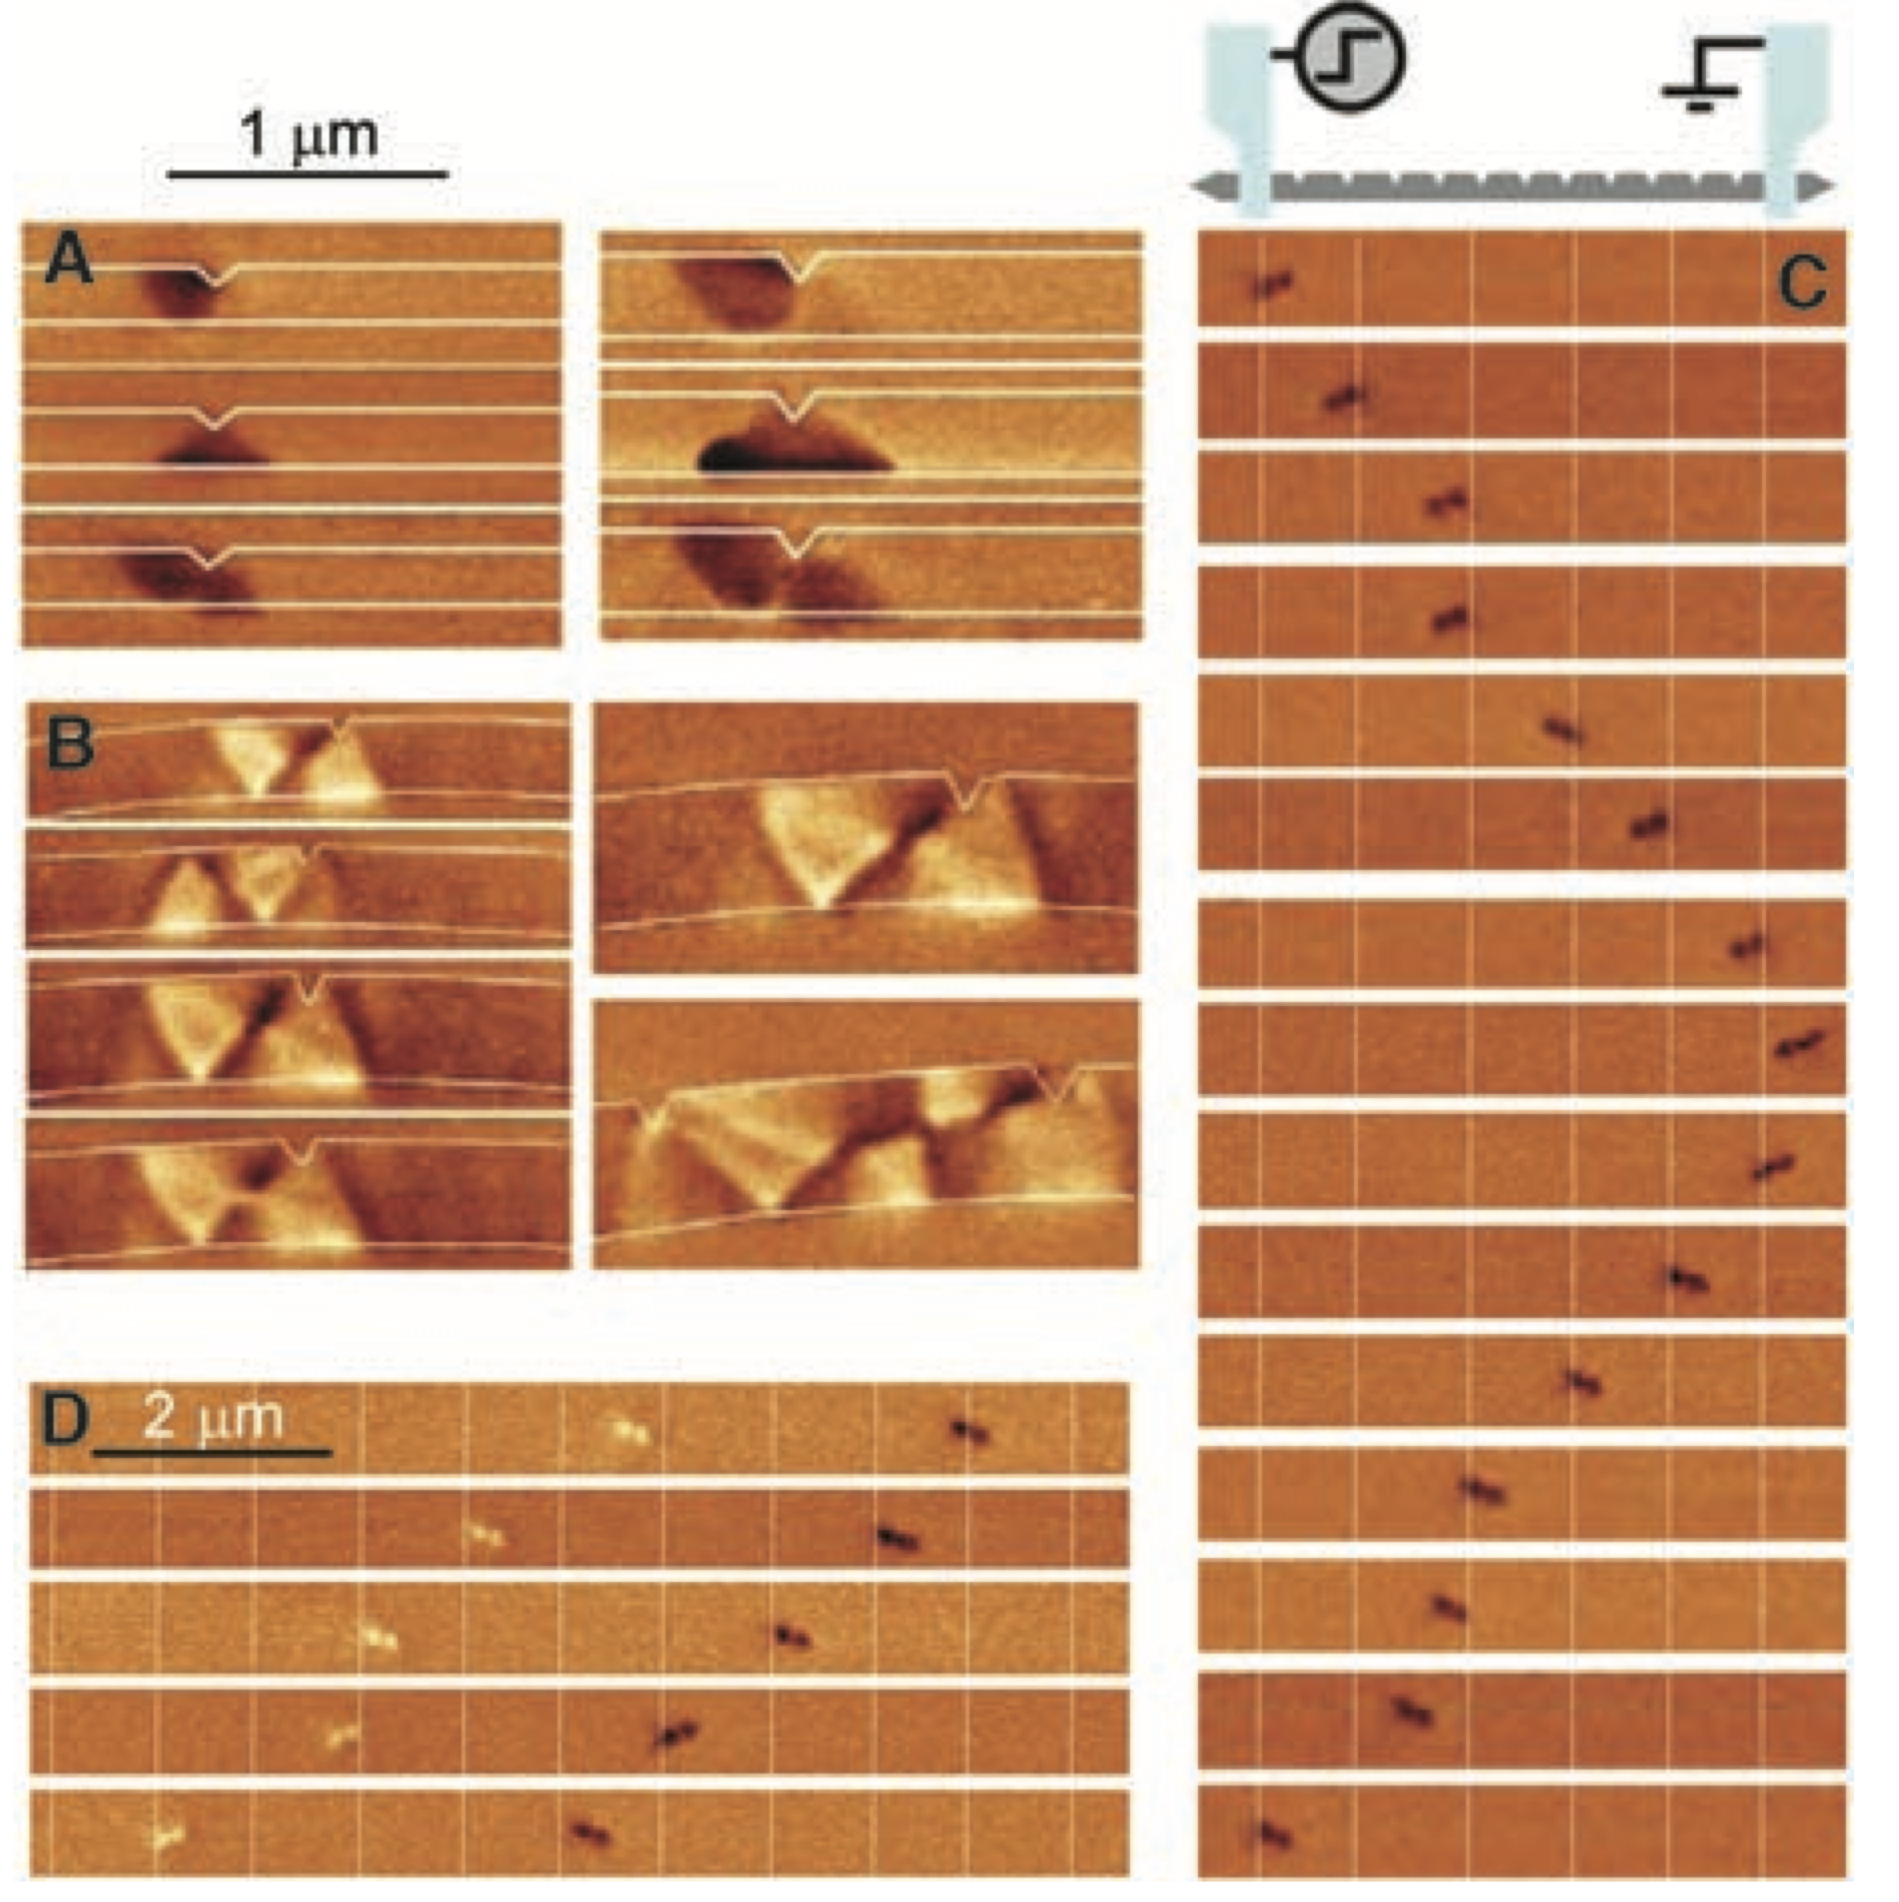
\includegraphics[width=0.6\linewidth]{../figs/DomainWalls}\\
{\small Measured structure of domain walls (taken from Parkin et al.).}
\end{center}


\section*{Short description}
Magnetic domain walls are formed at the boundaries between magnetic domains magnetized in opposite directions (up or down) along a so-called racetrack. The racetrack is a ferromagnetic nanowire, with data encoded as a pattern of magnetic domains along a portion of the wire. Using pulses of highly spin-polarized current to move the entire pattern of domain walls coherently along the length of the wire past read and write elements is a possible technology for future computer memory.


\section*{Mathematical Background}
The dynamics of the magnetization vector $\vec{m}$ is given by the Landau-Lifshitz equation
$$
\vec{m}\times\partial_t \vec{m}+\alpha \partial_t \vec{m}+\nabla E_\kappa(\vec{m})(1-\vec{m}\vec{m}^T) = h(1-\vec{m}\vec{m}^T).
$$
The magnetization vector is a unit vecor. The functional $E_\kappa(\vec{m})$ is the (reduced) internal micromagnetic energy which consists of
the exchange energy from spin interaction, anisotropy energy because of an external magnetic field, and magnetostatic interaction (Melcher 2004). 
Under proper assumptions, this equation allows for traveling wave solutions of domain walls. This means that the domain wall becomes unstable and moves. 


\section*{The Challenge}
%
\begin{itemize}
\item Develop numerical tools to study the structure of domain walls (e.g.\ Bloch walls)
\item Develop a simulation model for the dynamics of one-dimensional domain walls
\item Reproduce the theoretical and experimental results from the literature
\item Develop and implement a control strategy to move domain walls by an external magnetic field or by an external current
\end{itemize}
	


\section*{Literature}
%
\begin{itemize}
\item C.J.\ Garcia-Cervera, \emph{One-dimensional magnetic domain walls}, European Journal of Applied Mathematics 15 (2004) 451--486.
\item C.J.\ Garcia-Cervera, \emph{Numerical Micromagnetics: A Review}, Bol. Soc. Esp. Mat. Apl. 39 (2007) 103--135.
\item A.\ Hubert, R.\ Sch\"afer, \emph{Magnetic Domains: The Analysis of Magnetic Microstructures}, Springer-Verlag (1998).
\item C.\ Melcher, \emph{Domain wall motion in ferromagnetic layers}, Phys. D 192 (2004) 249--264.
\item S.S.P.\ Parkin, M.\ Hayashi, L.\ Thomas, \emph{Magnetic Domain-Wall Racetrack Memory}, Science 320 (2008) 190-194.
\end{itemize}
	












\end{document}
% ----------------------------------------------------------%


